\documentclass{standalone}

\usepackage{tikz}

\usetikzlibrary{calc}
\usetikzlibrary{positioning}
\usetikzlibrary{decorations}
\usetikzlibrary{decorations.markings}
\usetikzlibrary{decorations.text}

\begin{document}
  %noformat{
  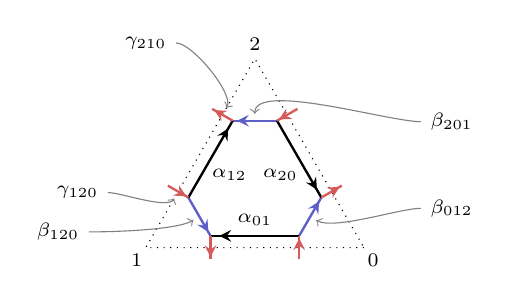
\begin{tikzpicture}
    \tikzstyle{e} = [postaction=decorate, decoration={markings, mark=at position 0.9 with {\arrow{stealth}}}, line width=0.3mm]
    % \tikzstyle{e} = [line width=0.3mm]
    \tikzstyle{r} = [color=red!70!darkgray!70]
    \tikzstyle{b} = [color=blue!60!darkgray!70]
    \tikzstyle{p} = [line width=0.3mm]

    \tikzset{font=\scriptsize}

    \coordinate[label={[label distance=6pt]330:{$0$}}] (v0) at (330:1.3);
    \coordinate[label={[label distance=6pt]210:{$1$}}] (v1) at (210:1.3);
    \coordinate[label={[label distance=8pt] 90:{$2$}}] (v2) at ( 90:1.3);

    \coordinate[                                     ] (v1p) at ($ (150:1.6) + (270:1.3) $);
    \coordinate[                                     ] (v2p) at ($ (150:1.6) + ( 30:1.3) $);
    % \coordinate[label={[label distance=6pt]150:{$3$}}] (v3p) at ($ (150:1.6) + (150:1.3) $);
    \coordinate[                                     ] (v3p) at ($ (150:1.6) + (150:1.3) $);

    \coordinate[                                     ] (v2q) at ($ ( 30:1.6) + (150:1.3) $);
    \coordinate[                                     ] (v0q) at ($ ( 30:1.6) + (270:1.3) $);
    % \coordinate[label={[label distance=6pt] 30:{$4$}}] (v4q) at ($ ( 30:1.6) + ( 30:1.3) $);
    \coordinate[                                     ] (v4q) at ($ ( 30:1.6) + ( 30:1.3) $);

    \coordinate[                                     ] (v1r) at ($ (270:1.6) + (150:1.3) $);
    \coordinate[                                     ] (v0r) at ($ (270:1.6) + ( 30:1.3) $);
    % \coordinate[label={[label distance=6pt]270:{$5$}}] (v5r) at ($ (270:1.6) + (270:1.3) $);
    \coordinate[                                     ] (v5r) at ($ (270:1.6) + (270:1.3) $);

    \coordinate (v01) at ($ (v0)!0.25!(v1)  $);
    \coordinate (v02) at ($ (v0)!0.25!(v2)  $);
    \coordinate (v10) at ($ (v1)!0.25!(v0)  $);
    \coordinate (v12) at ($ (v1)!0.25!(v2)  $);
    \coordinate (v20) at ($ (v2)!0.25!(v0)  $);
    \coordinate (v21) at ($ (v2)!0.25!(v1)  $);

    \coordinate (v31p) at ($ (v3p)!0.25!(v1p)  $);
    \coordinate (v32p) at ($ (v3p)!0.25!(v2p)  $);
    \coordinate (v13p) at ($ (v1p)!0.25!(v3p)  $);
    \coordinate (v12p) at ($ (v1p)!0.25!(v2p)  $);
    \coordinate (v23p) at ($ (v2p)!0.25!(v3p)  $);
    \coordinate (v21p) at ($ (v2p)!0.25!(v1p)  $);

    \coordinate (v02q) at ($ (v0q)!0.25!(v2q)  $);
    \coordinate (v20q) at ($ (v2q)!0.25!(v0q)  $);
    \coordinate (v04q) at ($ (v0q)!0.25!(v4q)  $);
    \coordinate (v40q) at ($ (v4q)!0.25!(v0q)  $);
    \coordinate (v24q) at ($ (v2q)!0.25!(v4q)  $);
    \coordinate (v42q) at ($ (v4q)!0.25!(v2q)  $);

    \coordinate (v01r) at ($ (v0r)!0.25!(v1r)  $);
    \coordinate (v10r) at ($ (v1r)!0.25!(v0r)  $);
    \coordinate (v51r) at ($ (v5r)!0.25!(v1r)  $);
    \coordinate (v15r) at ($ (v1r)!0.25!(v5r)  $);
    \coordinate (v05r) at ($ (v0r)!0.25!(v5r)  $);
    \coordinate (v50r) at ($ (v5r)!0.25!(v0r)  $);

    \draw[e, b] (v01) to (v02);
    \draw[e, b] (v12) to (v10);
    \draw[e, b] (v20) to (v21);
    \draw[e] (v01) to node[pos=0.5, above] (a01) {$\alpha_{01}$} (v10);
    \draw[e] (v20) to node[pos=0.7, left ] (a02) {$\alpha_{20}$} (v02);
    \draw[e] (v12) to node[pos=0.3, right] (a12) {$\alpha_{12}$} (v21);
    % \draw[e] (v01) -- (v10);
    % \draw[e] (v20) -- (v02);
    % \draw[e] (v12) -- (v21);

    \draw[dotted] ($ (v0) + (330:0.3) $) -- 
                  ($ (v1) + (210:0.3) $) -- 
                  ($ (v2) + ( 90:0.3) $) -- cycle;
    % \draw[dotted] ($ (v2) + ( 90:0.3) $) -- 
    %               ($ (v3p)+ (150:0.3) $) -- 
    %               ($ (v1) + (210:0.3) $);
    % \draw[dotted] ($ (v2) + ( 90:0.3) $) -- 
    %               ($ (v4q)+ ( 30:0.3) $) -- 
    %               ($ (v0) + (330:0.3) $);
    % \draw[dotted] ($ (v1) + (210:0.3) $) -- 
    %               ($ (v5r)+ (270:0.3) $) -- 
    %               ($ (v0) + (330:0.3) $);

    % \draw[p, b] (v32p) to (v31p);
    % \draw[p, b] (v13p) to (v12p);
    % \draw[p, b] (v21p) to (v23p);
    % \draw[p] (v13p) to (v31p);
    % \draw[p] (v32p) to (v23p);
    % \draw[p] (v21p) to (v12p);

    % \draw[p, b] (v42q) to (v40q);
    % \draw[p, b] (v04q) to (v02q);
    % \draw[p, b] (v20q) to (v24q);
    % \draw[p] (v04q) to (v40q);
    % \draw[p] (v42q) to (v24q);
    % \draw[p] (v20q) to (v02q);

    % \draw[p, b] (v51r) to (v50r);
    % \draw[p, b] (v05r) to (v01r);
    % \draw[p, b] (v10r) to (v15r);
    % \draw[p] (v05r) to (v50r);
    % \draw[p] (v51r) to (v15r);
    % \draw[p] (v10r) to (v01r);

    \draw[e, r] (v21) -- (v21p);
    \draw[e, r] (v12p) -- (v12);

    \draw[e, r] (v02) -- (v02q);
    \draw[e, r] (v20q) -- (v20);

    \draw[e, r] (v10) -- (v10r);
    \draw[e, r] (v01r) -- (v01);

    \node (b012) at ($ (  0:2.5) + (270:0.3) $) {$\beta_{012}$};
    \node (b120) at ($ (180:2.5) + (270:0.6) $) {$\beta_{120}$};
    \node (b201) at ($ (  0:2.5) + ( 90:0.8) $) {$\beta_{201}$};
    \draw[->, looseness=0.5, gray] (b012) to[out=180, in=330] (330:0.9);
    \draw[->, looseness=0.5, gray] (b201) to[out=180, in= 90] ( 90:0.9);
    \draw[->, looseness=0.5, gray] (b120) to[out=  0, in=210] (210:0.9);

    \node (g210) at ($ (150:1.6) + ( 90:1.0)             $) {$\gamma_{210}$};
    \node (g120) at ($ (150:1.6) + (210:1.0) + (270:0.4) $) {$\gamma_{120}$};
    \draw[->, looseness=0.5, gray] (g210) to[out=0, in= 60] ($ (v21)!0.5!(v21p) + ( 60:0.1) $);
    \draw[->, looseness=0.5, gray] (g120) to[out=0, in=240] ($ (v12)!0.5!(v12p) + (240:0.1) $);

    % \node (t201) at ($ (v20) + (355:0.9) $) {$\tau^{201}$};
    % \node (t021) at ($ (v02) + (  5:1.1) $) {$\tau^{021}$};
    % \draw[->, looseness=0.5, gray] (t201) to[out=180, in=  5] ($ (v20) + (0:0.05) $);
    % \draw[->, looseness=0.5, gray] (t021) to[out=180, in=355] ($ (v02) + (0:0.05) $);
  \end{tikzpicture}
  %}noformat
\end{document}
